\documentclass[aspectratio=169]{beamer}

% Packages
\usepackage[utf8]{inputenc}
\usepackage{tikz}
\usepackage{pgfplots}
\usepackage{amsmath}
\usepackage{booktabs}
\usetikzlibrary{arrows,calc}

% Theme Settings
\usetheme{Madrid}
\usecolortheme{beaver}
\setbeamertemplate{navigation symbols}{}

% Title Info
\title{Unit 5: Long-Run Consequences of Stabilization Policies}
\subtitle{The Phillips Curve, Money Growth, Deficits, and Economic Growth}
\author{Doğukan Günkördü}
\date{}

\begin{document}

% Title Slide
\begin{frame}
    \titlepage
\end{frame}

% Table of Contents
\begin{frame}{Unit 5 Overview}
    \tableofcontents
\end{frame}

% ==========================================
% SECTION 1: FISCAL & MONETARY POLICY ACTIONS
% ==========================================
\section{Fiscal and Monetary Policy Actions in the Short Run}

\begin{frame}{Review: Stabilization Policies}
    \begin{block}{Fiscal Policy (Congress \& President)}
        \begin{itemize}
            \item \textbf{Tools:} Government Spending ($G$), Taxes ($T$).
            \item \textbf{Expansionary:} $\uparrow G$ or $\downarrow T$ $\rightarrow$ $\uparrow$ AD.
            \item \textbf{Contractionary:} $\downarrow G$ or $\uparrow T$ $\rightarrow$ $\downarrow$ AD.
        \end{itemize}
    \end{block}
    
    \begin{block}{Monetary Policy (The Federal Reserve)}
        \begin{itemize}
            \item \textbf{Tools:} Reserve Requirement, Discount Rate, Open Market Operations, Interest on Reserves.
            \item \textbf{Expansionary:} $\uparrow$ Money Supply $\rightarrow$ $\downarrow$ Nominal Interest Rates $\rightarrow$ $\uparrow$ I $\rightarrow$ $\uparrow$ AD.
            \item \textbf{Contractionary:} $\downarrow$ Money Supply $\rightarrow$ $\uparrow$ Nominal Interest Rates $\rightarrow$ $\downarrow$ I $\rightarrow$ $\downarrow$ AD.
        \end{itemize}
    \end{block}
\end{frame}

\begin{frame}{Combined Policy Effects}
    What happens when Fiscal and Monetary policies work together?
    
    \begin{table}[]
        \centering
        \begin{tabular}{@{}llccc@{}}
            \toprule
            \textbf{Fiscal} & \textbf{Monetary} & \textbf{Aggregate Demand} & \textbf{Price Level} & \textbf{Real GDP} \\ \midrule
            Expansionary & Expansionary & \textbf{Increases} ($\uparrow\uparrow$) & $\uparrow$ & $\uparrow$ \\
            Contractionary & Contractionary & \textbf{Decreases} ($\downarrow\downarrow$) & $\downarrow$ & $\downarrow$ \\
            Expansionary & Contractionary & Indeterminate & Indeterminate & Indeterminate \\ 
            \bottomrule
        \end{tabular}
    \end{table}
    \vspace{0.5cm}
    \small{\textit{Note: When policies conflict (e.g., Exp Fiscal + Con Monetary), the change in AD depends on the relative magnitude of the shifts. However, interest rates will definitely rise.}}
\end{frame}

% ==========================================
% SECTION 2: THE PHILLIPS CURVE
% ==========================================
\section{The Phillips Curve}

\begin{frame}{The Short-Run Phillips Curve (SRPC)}
    The \textbf{Phillips Curve} illustrates the inverse relationship (trade-off) between the unemployment rate and the inflation rate in the short run.
    
    \begin{columns}
        \column{0.5\textwidth}
        \begin{itemize}
            \item \textbf{A.W. Phillips (1958):} Found that when unemployment is low, inflation tends to be high (and vice versa).
            \item \textbf{Logic:} Low unemployment $\rightarrow$ tight labor market $\rightarrow$ higher wages $\rightarrow$ higher prices.
        \end{itemize}
        
        \column{0.5\textwidth}
        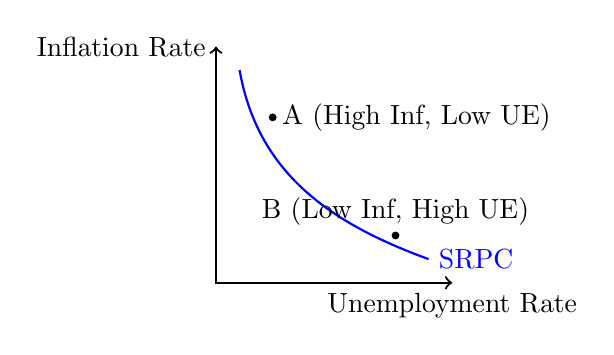
\begin{tikzpicture}[scale=0.6]
            \draw[thick, <->] (0,5) node[left]{Inflation Rate} -- (0,0) -- (5,0) node[below]{Unemployment Rate};
            \draw[thick, blue] (0.5,4.5) to [out=-80, in=160] (4.5,0.5) node[right]{SRPC};
            \filldraw (1.2, 3.5) circle (2pt) node[right]{A (High Inf, Low UE)};
            \filldraw (3.8, 1.0) circle (2pt) node[above]{B (Low Inf, High UE)};
        \end{tikzpicture}
    \end{columns}
\end{frame}

\begin{frame}{Linking AD shifts to the Phillips Curve}
    Changes in \textbf{Aggregate Demand} cause \textbf{movements along} the SRPC.
    
    \begin{columns}
        \column{0.5\textwidth}
        \centering
        \textbf{AD/AS Model}\\
        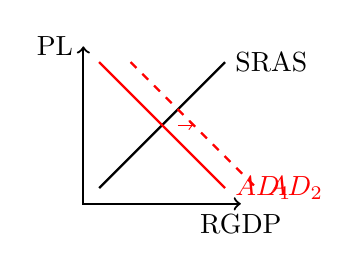
\begin{tikzpicture}[scale=0.4]
            \draw[thick, <->] (0,5) node[left]{PL} -- (0,0) -- (5,0) node[below]{RGDP};
            \draw[thick] (0.5,0.5) -- (4.5,4.5) node[right]{SRAS};
            \draw[thick, red] (0.5,4.5) -- (4.5,0.5) node[right]{$AD_1$};
            \draw[thick, red, dashed] (1.5,4.5) -- (5.5,0.5) node[right]{$AD_2$};
            \draw[->, red] (3,2.5) -- (3.5,2.5);
        \end{tikzpicture}
        
        \column{0.5\textwidth}
        \centering
        \textbf{Phillips Curve}\\
        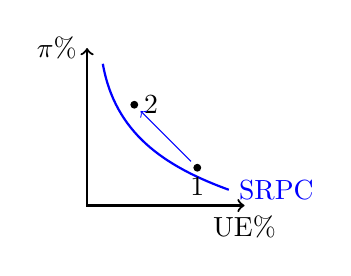
\begin{tikzpicture}[scale=0.4]
            \draw[thick, <->] (0,5) node[left]{$\pi\%$} -- (0,0) -- (5,0) node[below]{UE\%};
            \draw[thick, blue] (0.5,4.5) to [out=-80, in=160] (4.5,0.5) node[right]{SRPC};
            \filldraw (3.5, 1.2) circle (3pt) node[below]{1};
            \filldraw (1.5, 3.2) circle (3pt) node[right]{2};
            \draw[->, blue] (3.3, 1.4) -- (1.7, 3.0);
        \end{tikzpicture}
    \end{columns}
    \vspace{0.5cm}
    \textbf{Key Rule:} If AD shifts Right $\rightarrow$ Unemployment falls, Inflation rises $\rightarrow$ Slide UP the SRPC.
\end{frame}

\begin{frame}{Shifting the SRPC}
    Changes in \textbf{Short-Run Aggregate Supply (SRAS)} cause the \textbf{SRPC to shift}.
    
    \begin{columns}
        \column{0.5\textwidth}
        \begin{itemize}
            \item \textbf{Supply Shock:} A negative supply shock (e.g., oil prices $\uparrow$) shifts SRAS left.
            \item \textbf{Stagflation:} Price Level $\uparrow$ AND Unemployment $\uparrow$.
            \item The trade-off worsens; the SRPC shifts \textbf{Right}.
        \end{itemize}
        
        \column{0.5\textwidth}
        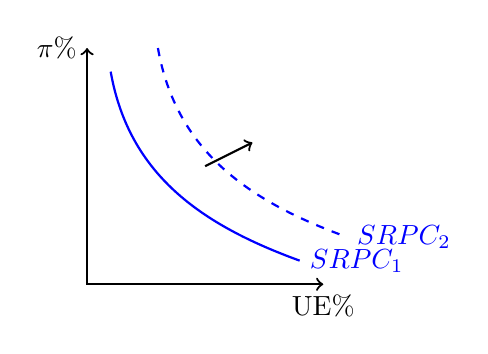
\begin{tikzpicture}[scale=0.6]
            \draw[thick, <->] (0,5) node[left]{$\pi\%$} -- (0,0) -- (5,0) node[below]{UE\%};
            \draw[thick, blue] (0.5,4.5) to [out=-80, in=160] (4.5,0.5) node[right]{$SRPC_1$};
            \draw[thick, blue, dashed] (1.5,5.0) to [out=-80, in=160] (5.5,1.0) node[right]{$SRPC_2$};
            \draw[->, thick] (2.5,2.5) -- (3.5,3.0);
        \end{tikzpicture}
    \end{columns}
    \vspace{0.2cm}
    \small{Note: SRAS Left = SRPC Right (Misery index increases).}
\end{frame}

\begin{frame}{The Long-Run Phillips Curve (LRPC)}
    In the long run, there is \textbf{no trade-off} between inflation and unemployment.
    
    \begin{columns}
        \column{0.5\textwidth}
        \begin{itemize}
            \item The economy gravitates toward the \textbf{Natural Rate of Unemployment (NRU)}.
            \item The LRPC is vertical at the NRU.
            \item \textbf{Monetary Neutrality:} In the long run, increasing the money supply only creates inflation; it does not lower unemployment.
        \end{itemize}
        
        \column{0.5\textwidth}
        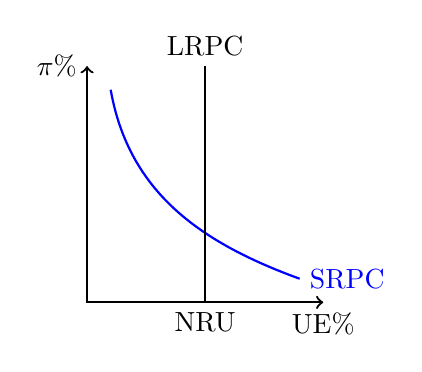
\begin{tikzpicture}[scale=0.6]
            \draw[thick, <->] (0,5) node[left]{$\pi\%$} -- (0,0) -- (5,0) node[below]{UE\%};
            \draw[thick, blue] (0.5,4.5) to [out=-80, in=160] (4.5,0.5) node[right]{SRPC};
            \draw[thick, black] (2.5, 0) -- (2.5, 5) node[above]{LRPC};
            \draw[dashed] (2.5,0) node[below]{NRU};
        \end{tikzpicture}
    \end{columns}
\end{frame}

% ==========================================
% SECTION 3: MONEY GROWTH AND INFLATION
% ==========================================
\section{Money Growth and Inflation}

\begin{frame}{The Quantity Theory of Money}
    Based on the \textbf{Equation of Exchange} (Irving Fisher):
    
    \begin{block}{The Equation}
        \[ M \times V = P \times Y \]
    \end{block}
    
    \begin{description}
        \item[M] = Money Supply (M1 or M2)
        \item[V] = Velocity of Money (How many times a dollar is spent per year)
        \item[P] = Price Level
        \item[Y] = Real GDP (Output)
        \item[P $\times$ Y] = Nominal GDP
    \end{description}
\end{frame}

\begin{frame}{Assumptions and Implications}
    \begin{itemize}
        \item \textbf{Velocity (V)} is assumed to be relatively stable in the short run.
        \item \textbf{Real Output (Y)} is determined by resources and technology (not money) in the long run.
    \end{itemize}
    
    \vspace{0.5cm}
    
    \textbf{The Conclusion:}
    If $V$ and $Y$ are constant, changes in the Money Supply ($M$) translate directly to changes in the Price Level ($P$).
    
    \[ \uparrow M \Rightarrow \uparrow P \]
    
    \begin{alertblock}{Monetary Neutrality}
        In the long run, changes in the money supply affect \textbf{nominal} variables (prices, wages) but NOT \textbf{real} variables (Real GDP, employment).
    \end{alertblock}
\end{frame}

\begin{frame}{Hyperinflation}
    \begin{itemize}
        \item If the central bank increases the money supply significantly faster than the growth of Real GDP ($Y$), the result is \textbf{inflation}.
        \item \textbf{Hyperinflation:} Rapid, excessive, and out-of-control price increases (e.g., Brazil in the 1990s, Zimbabwe).
        \item Caused by governments printing money to pay debts (seigniorage) without underlying economic growth.
    \end{itemize}
\end{frame}

% ==========================================
% SECTION 4: CROWDING OUT
% ==========================================
\section{Crowding Out}

\begin{frame}{What is Crowding Out?}
    \begin{itemize}
        \item \textbf{Definition:} The decrease in investment spending ($I$) and consumer spending ($C$) that occurs when the government borrows to finance a budget deficit.
        \item \textbf{The Chain Reaction:}
        \begin{enumerate}
            \item Government runs a deficit $\rightarrow$ must borrow funds.
            \item Demand for Loanable Funds increases ($\uparrow D_{LF}$) OR Supply of Loanable Funds decreases ($\downarrow S_{LF}$).
            \item \textbf{Real Interest Rates rise} ($\uparrow r$).
            \item Private investment is "crowded out" because it is more expensive to borrow.
        \end{enumerate}
        \item \textbf{Long-Run Impact:} Less investment $\rightarrow$ lower rate of physical capital accumulation $\rightarrow$ slower economic growth.
    \end{itemize}
\end{frame}

\begin{frame}{Modeling Crowding Out (Loanable Funds Market)}
    \begin{columns}
        \column{0.5\textwidth}
        \begin{itemize}
            \item \textbf{Shift:} Government borrowing shifts $D_{LF}$ to the right.
            \item \textbf{Result:} Equilibrium real interest rate increases from $r_1$ to $r_2$.
            \item \textbf{Impact:} Higher interest rates discourage businesses from buying machinery/tools (Investment).
        \end{itemize}
        
        \column{0.5\textwidth}
        \centering
        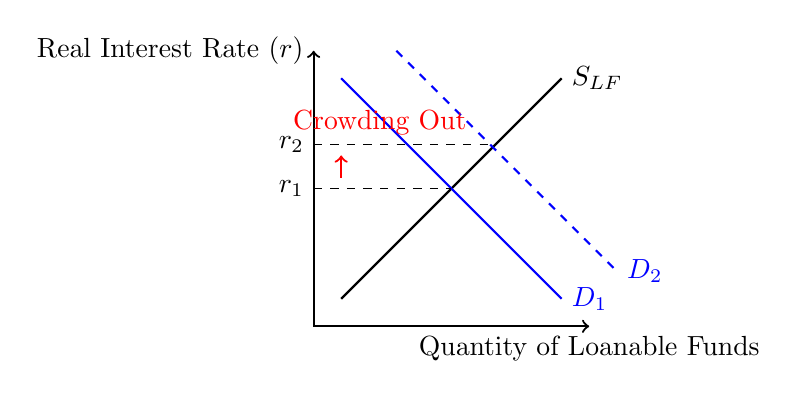
\begin{tikzpicture}[scale=0.7]
            \draw[thick, <->] (0,5) node[left]{Real Interest Rate ($r$)} -- (0,0) -- (5,0) node[below]{Quantity of Loanable Funds};
            \draw[thick] (0.5,0.5) -- (4.5,4.5) node[right]{$S_{LF}$};
            \draw[thick, blue] (0.5,4.5) -- (4.5,0.5) node[right]{$D_1$};
            \draw[thick, blue, dashed] (1.5,5.0) -- (5.5,1.0) node[right]{$D_2$};
            
            \draw[dashed] (0,2.5) node[left]{$r_1$} -- (2.5,2.5);
            \draw[dashed] (0,3.3) node[left]{$r_2$} -- (3.3,3.3);
            \draw[->, thick, red] (0.5,2.7) -- (0.5,3.1);
            \node[red] at (1.2,3.7) {Crowding Out};
        \end{tikzpicture}
    \end{columns}
\end{frame}

% ==========================================
% SECTION 5: DEFICITS AND DEBTS
% ==========================================
\section{Deficits and Debts}

\begin{frame}{Budget Deficits vs. National Debt}
    \begin{block}{Budget Deficit (A "Flow" Variable)}
        \begin{itemize}
            \item Occurs within a specific fiscal year.
            \item Tax Revenues $<$ Government Spending ($T < G$).
        \end{itemize}
    \end{block}
    
    \begin{block}{National Debt (A "Stock" Variable)}
        \begin{itemize}
            \item The accumulation of all past annual deficits and surpluses.
            \item Total amount the government owes to its creditors.
        \end{itemize}
    \end{block}
    
    \begin{itemize}
        \item \textbf{Sustainability:} National debt is often measured as a percentage of GDP. If debt grows faster than GDP, it can lead to higher taxes or reduced services in the future.
    \end{itemize}
\end{frame}

% ==========================================
% SECTION 6: ECONOMIC GROWTH
% ==========================================
\section{Economic Growth}

\begin{frame}{Defining Economic Growth}
    \begin{itemize}
        \item \textbf{Definition:} A sustained increase in a nation's \textbf{Real GDP per capita} over time.
        \item \textbf{Per Capita matters:} It accounts for population growth to measure changes in the standard of living.
        \item \textbf{The Aggregate Production Function:} Shows that output ($Y$) depends on:
        \begin{enumerate}
            \item \textbf{Physical Capital ($K$):} Human-made resources (factories, tools).
            \item \textbf{Human Capital ($L$):} Skills, education, and health of the workforce.
            \item \textbf{Natural Resources ($N$):} Land, minerals, water.
            \item \textbf{Technology ($A$):} Scientific knowledge and processes.
        \end{enumerate}
    \end{itemize}
\end{frame}

\begin{frame}{Graphing Growth: PPC and AD/AS}
    \begin{columns}
        \column{0.5\textwidth}
        \centering
        \textbf{Production Possibilities Curve}\\
        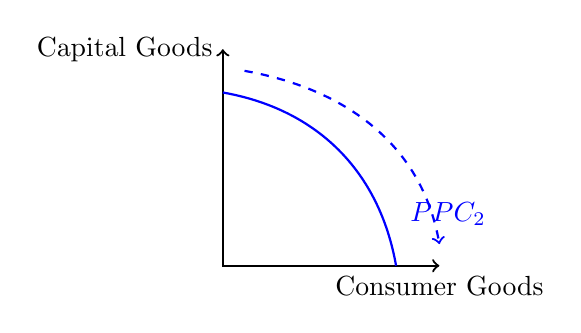
\begin{tikzpicture}[scale=0.55]
            \draw[thick, <->] (0,5) node[left]{Capital Goods} -- (0,0) -- (5,0) node[below]{Consumer Goods};
            \draw[thick, blue] (0,4) to [out=-10, in=100] (4,0);
            \draw[thick, blue, dashed, ->] (0.5,4.5) to [out=-10, in=100] (5,0.5);
            \node[blue] at (5.2,1.2) {$PPC_2$};
        \end{tikzpicture}
        
        \column{0.5\textwidth}
        \centering
        \textbf{Long-Run Aggregate Supply}\\
        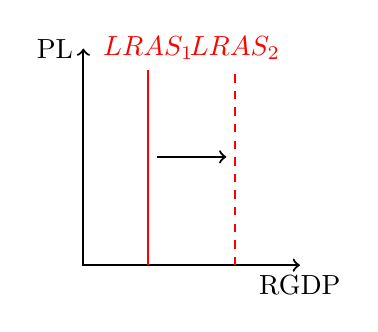
\begin{tikzpicture}[scale=0.55]
            \draw[thick, <->] (0,5) node[left]{PL} -- (0,0) -- (5,0) node[below]{RGDP};
            \draw[thick, red] (1.5,0) -- (1.5,4.5) node[above]{$LRAS_1$};
            \draw[thick, red, dashed] (3.5,0) -- (3.5,4.5) node[above]{$LRAS_2$};
            \draw[->, thick] (1.7,2.5) -- (3.3,2.5);
        \end{tikzpicture}
    \end{columns}
    \vspace{0.4cm}
    \centering \textbf{Economic Growth = Outward shift of the PPC and the LRAS curve.}
\end{frame}

% ==========================================
% SECTION 7: PUBLIC POLICY AND GROWTH
% ==========================================
\section{Public Policy and Economic Growth}

\begin{frame}{Supply-Side Policies to Promote Growth}
    Governments can incentivize growth by focusing on the determinants of the production function:
    
    \begin{itemize}
        \item \textbf{Physical Capital:} Incentives for investment (e.g., investment tax credits) and infrastructure spending.
        \item \textbf{Human Capital:} Public funding for \textbf{education} and job training programs.
        \item \textbf{Technology/R\&D:} Grants for scientific research and patent protections.
        \item \textbf{Supply-Side Tax Cuts:} Reducing marginal tax rates on business profits to encourage expansion and hiring.
    \end{itemize}
    
    \begin{alertblock}{The Trade-off}
        Many growth-oriented policies require deficit spending, which can lead to \textbf{Crowding Out}. The net effect on growth depends on whether the increase in productivity exceeds the decrease in private investment.
    \end{alertblock}
\end{frame}

% ==========================================
% UNIT SUMMARY
% ==========================================
\section{Unit 5 Summary}

\begin{frame}{Comprehensive Unit 5 Summary}
    \begin{enumerate}
        \item \textbf{Phillips Curve:} 
        \begin{itemize}
            \item \textbf{Short Run:} Inverse trade-off between Inflation and Unemployment.
            \item \textbf{Long Run:} Vertical curve at the NRU (No trade-off).
        \end{itemize}
        
        \item \textbf{Money and Inflation:}
        \begin{itemize}
            \item \textbf{Quantity Theory ($MV=PY$):} Rapid money growth $\rightarrow$ Inflation.
            \item \textbf{Monetary Neutrality:} Money affects prices, not real output, in the long run.
        \end{itemize}
        
        \item \textbf{Fiscal Friction:}
        \begin{itemize}
            \item \textbf{Crowding Out:} Deficit spending $\rightarrow$ Higher Interest Rates $\rightarrow$ Lower Private Investment.
        \end{itemize}
        
        \item \textbf{Economic Growth:}
        \begin{itemize}
            \item Defined as an increase in \textbf{Real GDP per Capita}.
            \item Driven by Human Capital, Physical Capital, and Technology.
            \item Shown by rightward shifts of LRAS and PPC.
        \end{itemize}
    \end{enumerate}
\end{frame}

\end{document}
